
\documentclass[14pt]{extarticle}
\usepackage{graphicx}
\usepackage{pdfpages}
\usepackage[T1]{fontenc}
\usepackage[margin=1in]{geometry}

\graphicspath{ {./edited_images/} }

\begin{document}
    \pagenumbering{arabic}
    \pagestyle{plain}

    \title{\Huge Assignment 6\\ Computer Networks}
    \author{\huge Vikas Gola : 2016UCS0023}
    \maketitle
    \newpage


    \begin{center}
        {\Large \textbf{SET 1: The Basic DNS }}
    \end{center}
    
    \noindent
    \textbf{\large Question 1}
    Determine which transport layer protocol was used for sending the DNS queries? 
    What are the benefits and drawbacks of using that protocol ?\\[10pt]
    \textbf{\large Answer}
    UDP (User Datagram protocol) was used for sending the DNS queries. The benefits of using UDP is that it is fast, efficient and lightweight.
    The one of the big drawbacks of UDP is that it does not support error recovery. The another drawback of UDP is that it does not give guarantee that 
    the messages or packets sent would reach at all.\\[10pt]
    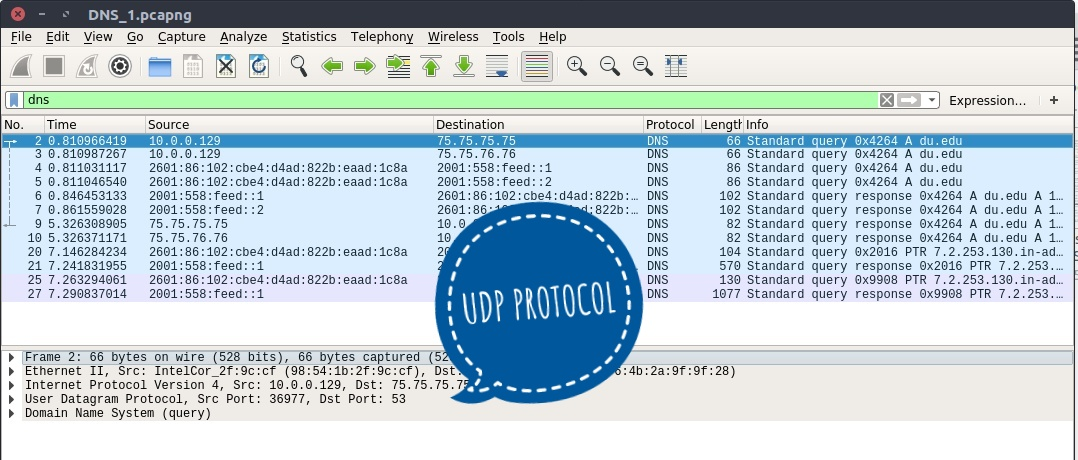
\includegraphics[scale=0.45]{1_1}
    \vspace{1cm}

    \noindent
    \textbf{\large Question 2}
    What port numbers are used for sending and receiving the packet in packet \#2 ?\\[10pt]
    \textbf{\large Answer}
    Source port: 36977\\
    Destination port: 53\\[10pt]
    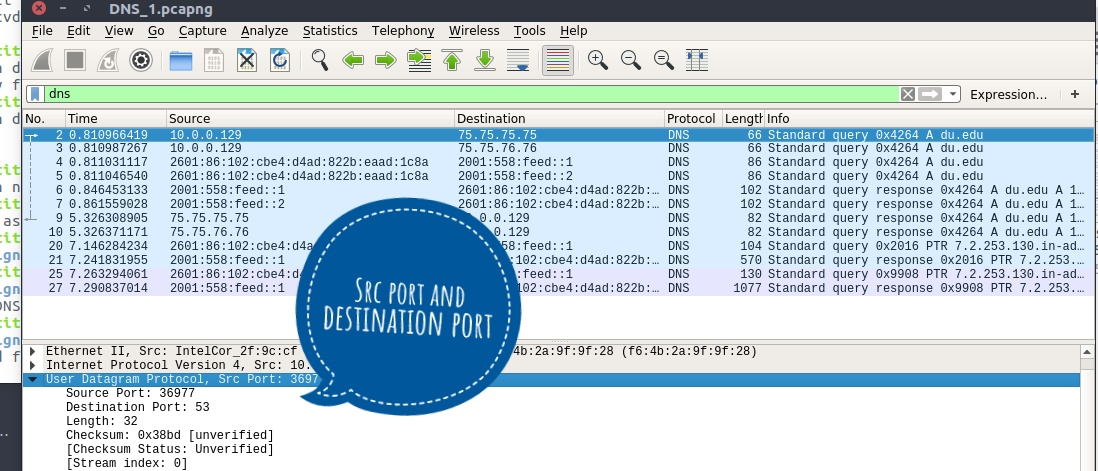
\includegraphics[scale=0.45]{1_2}
    \vspace{1cm}

    \noindent
    \textbf{\large Question 3}
    What is the destination address of packet \#2? What type of DNS query it is? 
    What type of DNS server it is? What flags are set in the query ?\\[10pt]
    \textbf{\large Answer}
    Destination address: 75.75.75.75\\
    It is a Recursive Query( 0x0100 Standard Query ). The DNS server type is authoritative server.\\
    Flags in the query are:\\
    0... .... .... .... = Response: Message is a query\\
    .000 0... .... .... = Opcode: Standard query (0)\\
    .... ..0. .... .... = Truncated: Message is not truncated\\
    .... ...1 .... .... = Recursion desired: Do query recursively\\
    .... .... .0.. .... = Z: reserved (0)\\
    .... .... ...0 .... = Non-authenticated data: Unacceptable\\[10pt]
    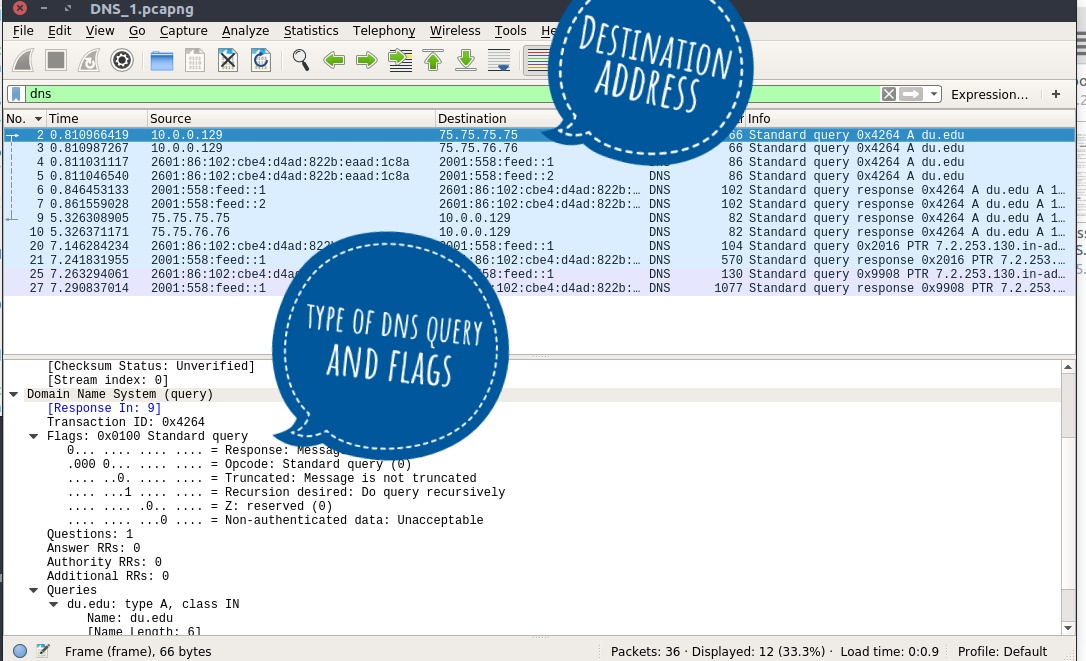
\includegraphics[scale=0.45]{1_3}
    \vspace{1cm}


    \noindent
    \textbf{\large Question 4}
    How many DNS servers are queried to for resolving the domain name du.edu.?\\[10pt]
    \textbf{\large Answer}
    1 DNS server is queried to for resolving the domain name du.edu.
    \vspace{1cm}

    \noindent
    \textbf{\large Question 5}
    Which packet contains the response of the query sent in packet \#2 ?  Which flags are set in the response?\\[10pt]
    \textbf{\large Answer}
    9th packet contains the response of query of packet \#2.\\
    Flags in the response are:\\
    1... .... .... .... = Response: Message is a response\\
    .000 0... .... .... = Opcode: Standard query (0)\\
    .... .0.. .... .... = Authoritative: Server is not an authority for domain\\
    .... ..0. .... .... = Truncated: Message is not truncated\\
    .... ...1 .... .... = Recursion desired: Do query recursively\\
    .... .... 1... .... = Recursion available: Server can do recursive queries\\
    .... .... .0.. .... = Z: reserved (0)\\
    .... .... ..0. .... = Answer authenticated: Answer/authority portion was not authenticated by the server\\
    .... .... ...0 .... = Non-authenticated data: Unacceptable\\
    .... .... .... 0000 = Reply code: No error (0)\\[10pt]
    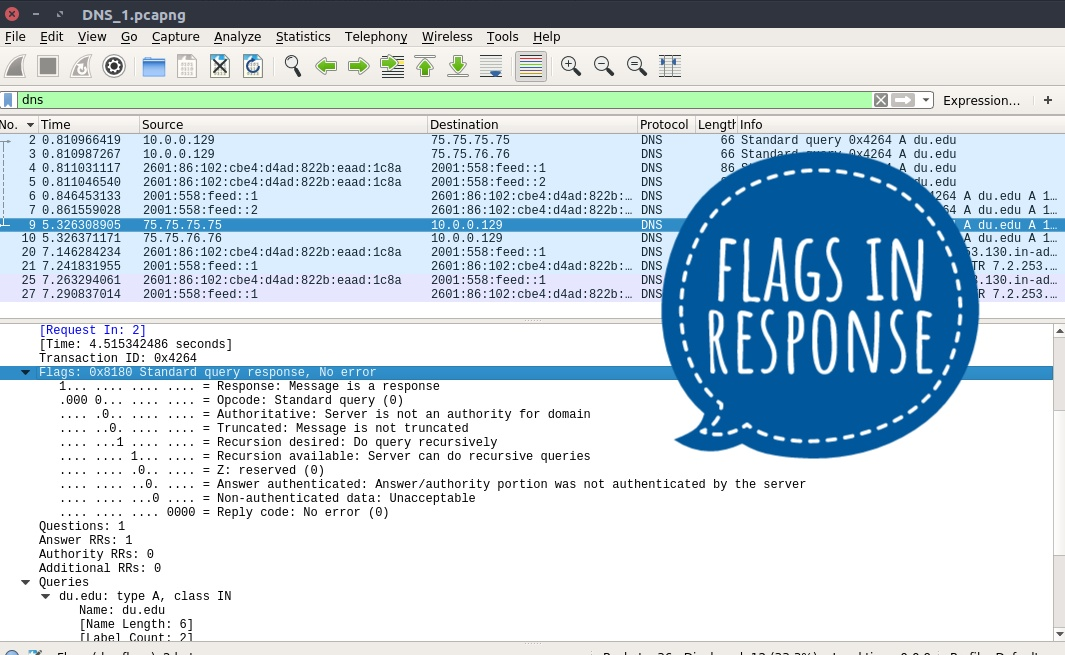
\includegraphics[scale=0.45]{1_5_1}\\[10pt]
    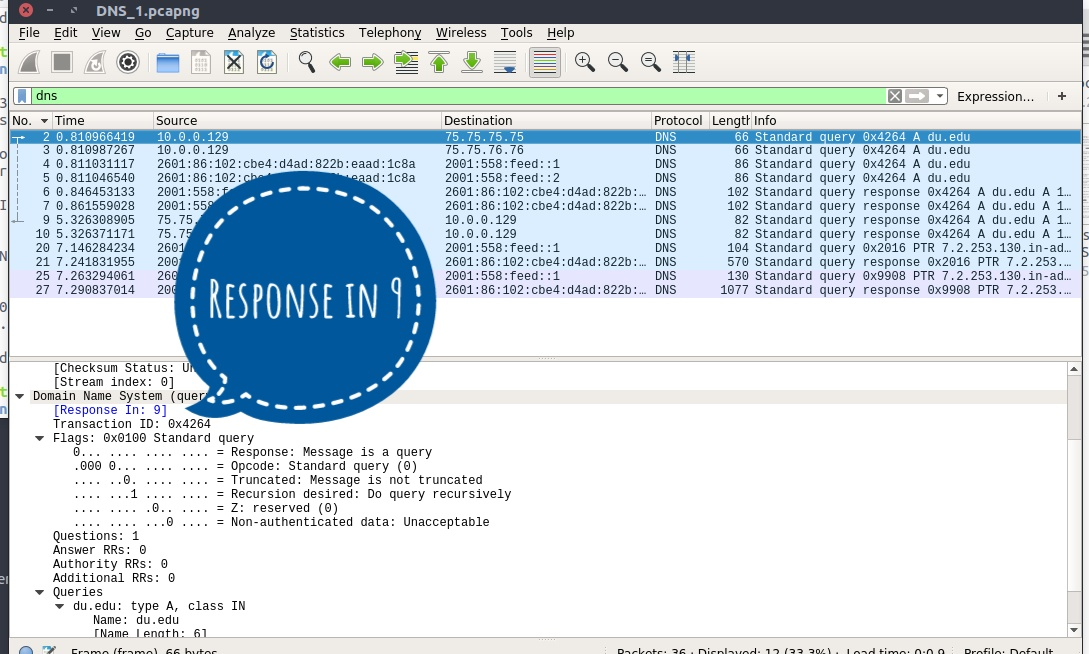
\includegraphics[scale=0.45]{1_5_2}
    \vspace{1cm}

    \noindent
    \textbf{\large Question 6}
    How many answers do you get in the response? Is the response from authoritative server ?\\[10pt]
    \textbf{\large Answer}
    1 answer in the response. No, response is not from Authoritative Server.\\[10pt]
    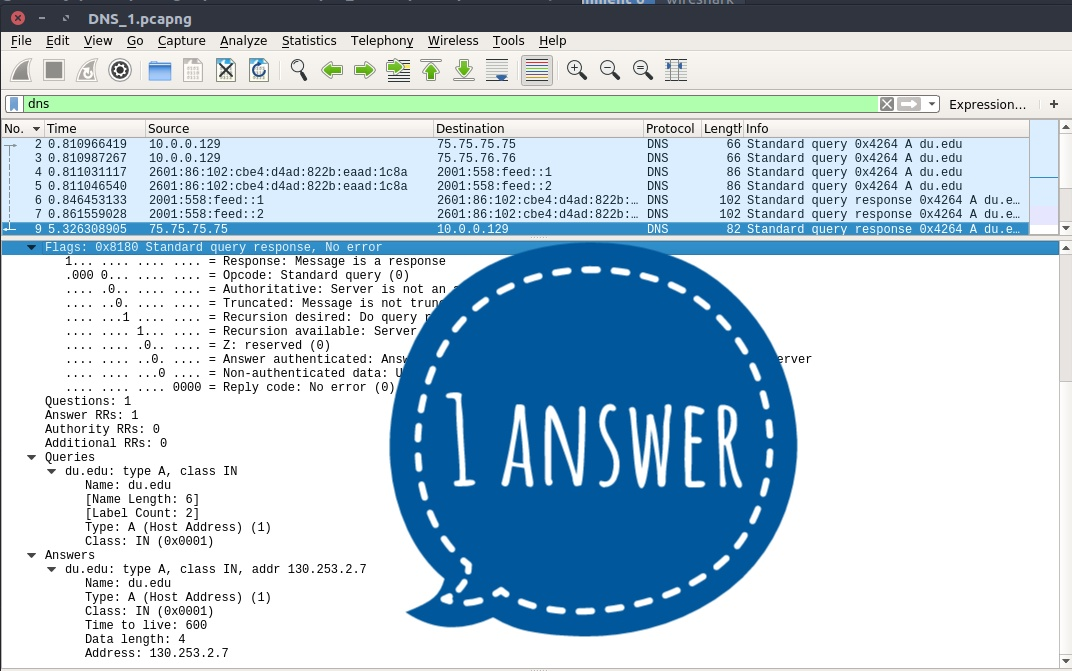
\includegraphics[scale=0.45]{1_6}
    \vspace{1cm}

    \noindent
    \textbf{\large Question 7}
    What does the query in the packet \#25 do?\\[10pt]
    \textbf{\large Answer}
    Query in the packet \#25 do inverse lookup of IP 7.2.253.130.\\[10pt]
    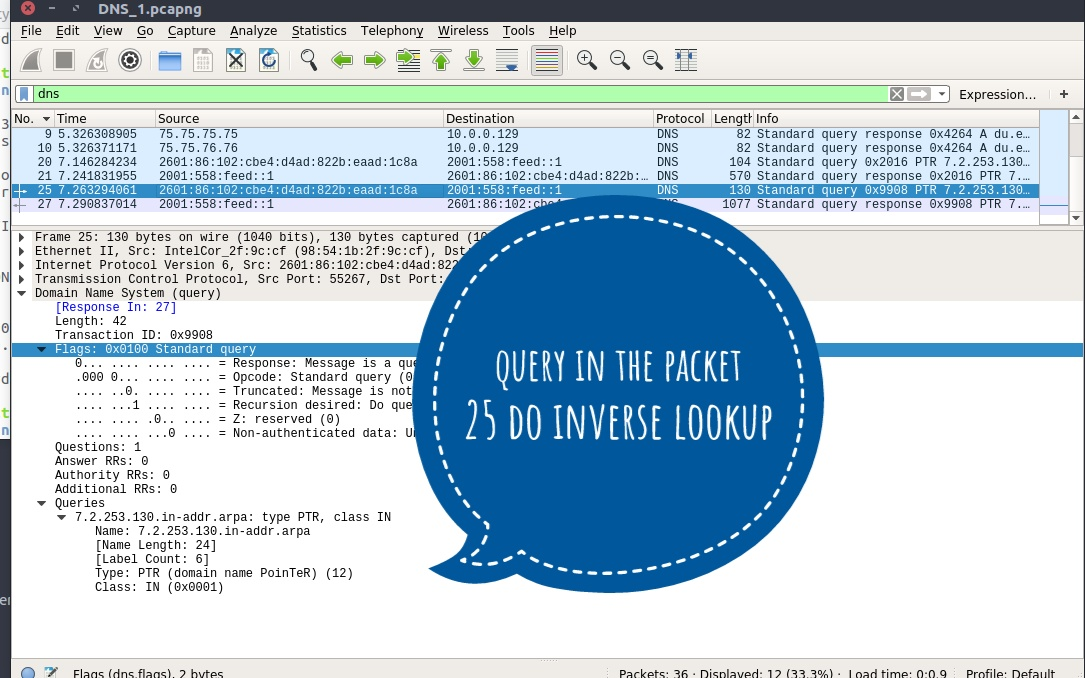
\includegraphics[scale=0.45]{1_7}
    \vspace{1cm}

    \noindent
    \textbf{\large Question 8}
    Which packet contains the response of the query sent? What is the response?\\[10pt]
    \textbf{\large Answer}
    Response of query of packet \#25 contains in packet \#27. The response is the answers of query in which some numbers of answers 
    which gives Domain Name corresponding to IP address which was quired.\\[10pt]
    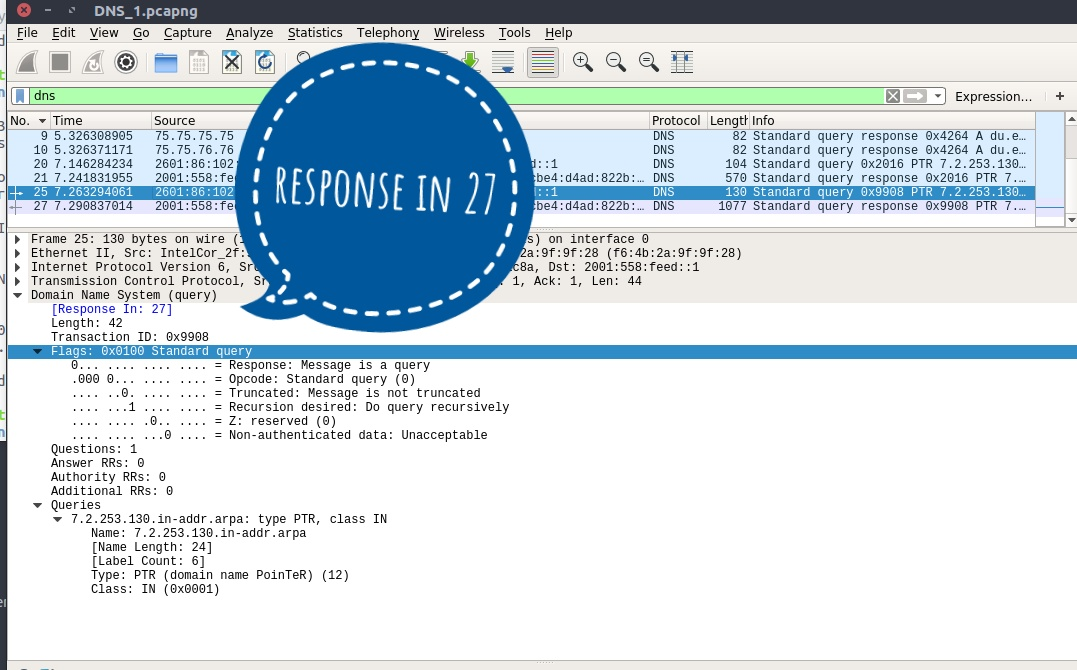
\includegraphics[scale=0.45]{1_8_1}\\[10pt]
    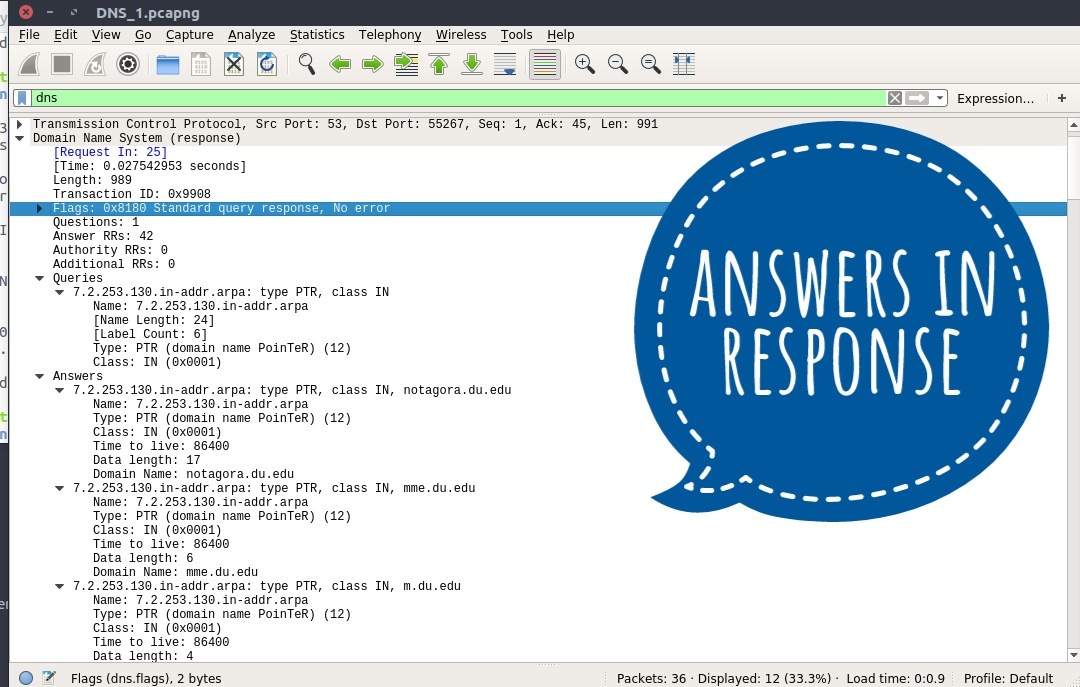
\includegraphics[scale=0.45]{1_8_2}
    \vspace{1cm}

    \begin{center}
        {\Large \textbf{SET 2: Using the DNS2.pcapng }}
    \end{center}

    \noindent
    \textbf{\large Question 1}
    In packet \#10, what is the destination IP address of the server? 
    To which DNS server request is being sent to?\\[10pt]
    \textbf{\large Answer}
    The destination IP address of the server is 208.78.70.24. The request has been sent to "cpnr-authdns-dhcp-vm-1.du.edu" DNS server\\[10pt]
    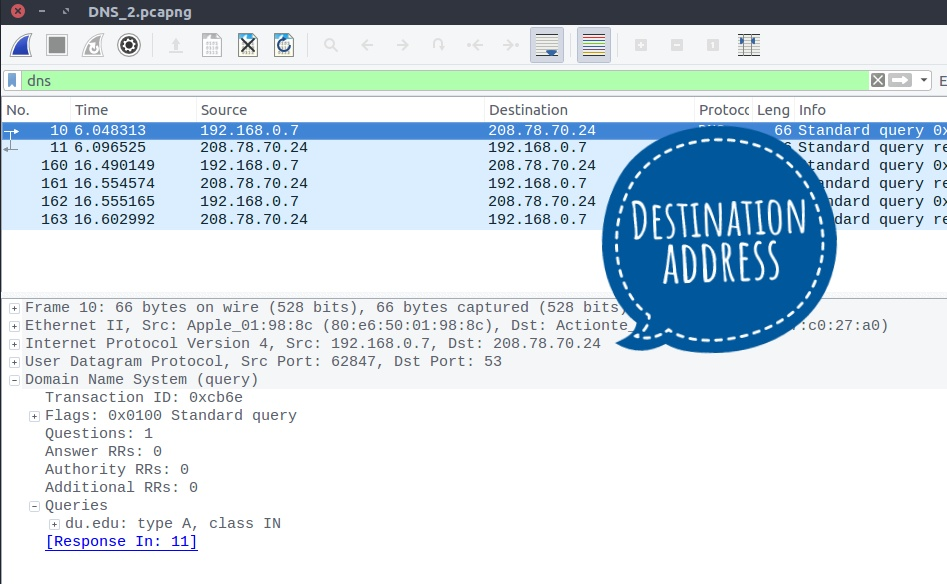
\includegraphics[scale=0.45]{2_1}\\[10pt]
    \vspace{1cm}

    \noindent
    \textbf{\large Question 2}
    Which packet contains the reply of the query that is sent in packet \#10?
    Did DNS server reply ? Examine the flags of the response and what you infer from the flags?\\[10pt]
    \textbf{\large Answer}
    Packet \#11 contains the reply of query that is sent in packet \#10. Yes, DNS server reply.\\
    Flags of the response are given below as follows which shows that request has been processed which any error:\\
    Flags: 0x8500 Standard query response, No error\\
    1... .... .... .... = Response: Message is a response\\
    .000 0... .... .... = Opcode: Standard query (0)\\
    .... .1.. .... .... = Authoritative: Server is an authority for domain\\
    .... ..0. .... .... = Truncated: Message is not truncated\\
    .... ...1 .... .... = Recursion desired: Do query recursively\\
    .... .... 0... .... = Recursion available: Server can't do recursive queries\\
    .... .... .0.. .... = Z: reserved (0)\\
    .... .... ..0. .... = Answer authenticated: Answer/authority portion was not authenticated by the server\\
    .... .... ...0 .... = Non-authenticated data: Unacceptable\\
    .... .... .... 0000 = Reply code: No error (0)\\[10pt]
    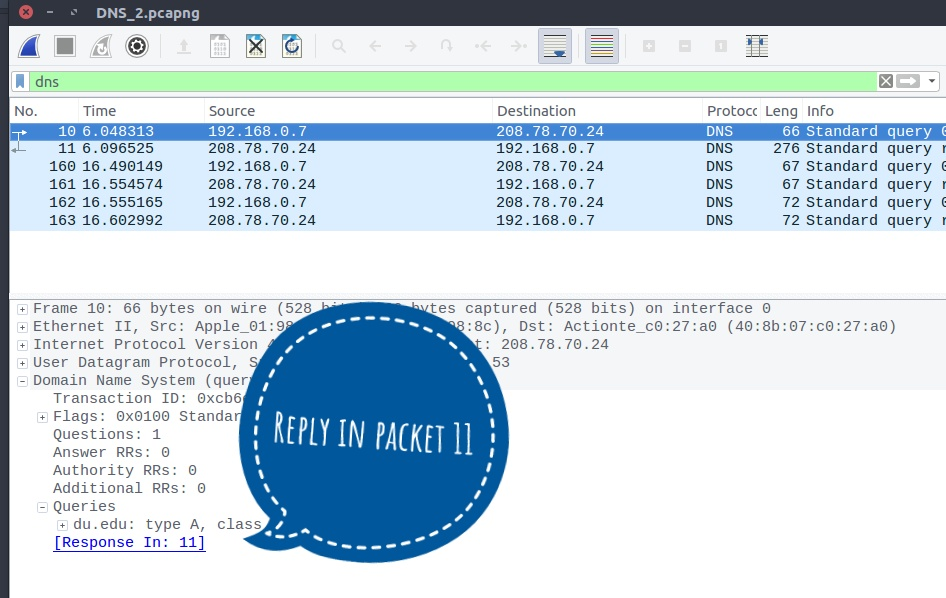
\includegraphics[scale=0.45]{2_2_1}\\[10pt] 
    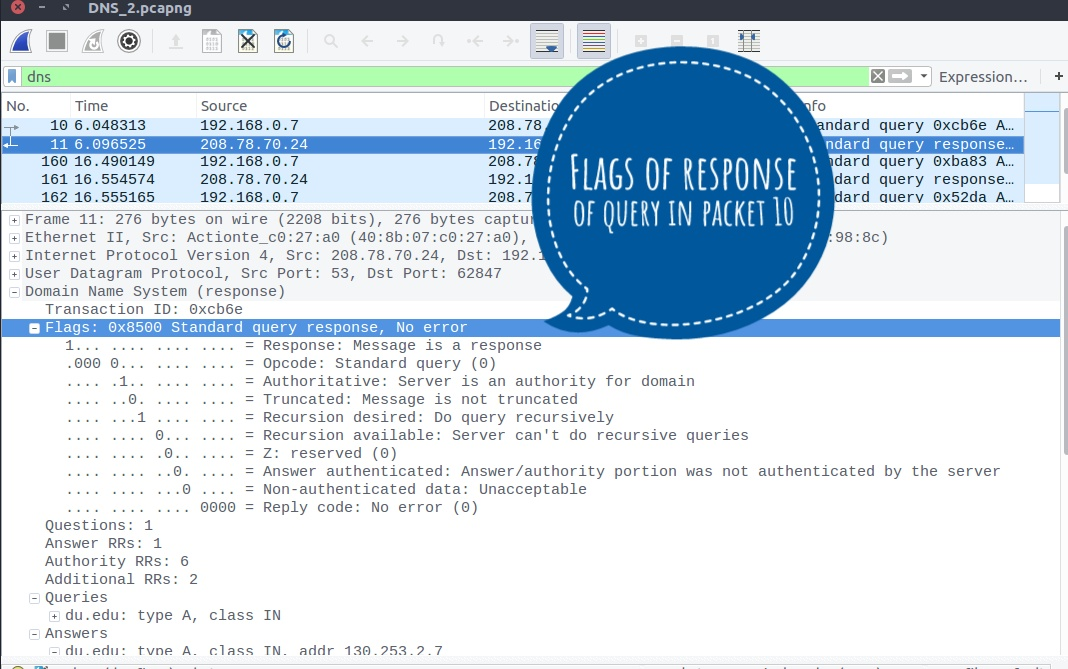
\includegraphics[scale=0.45]{2_2_2}\\[10pt] 
    \vspace{1cm}

    \noindent
    \textbf{\large Question 3}
    To which DNS server, is the DNS request in \#160 sent to? 
    What does the DNS request ask from the DNS server?\\[10pt]
    \textbf{\large Answer}
    The request in \#160 is sent to 208.78.70.24. DNS request ask for IP address of "mit.edu".\\[10pt]        
    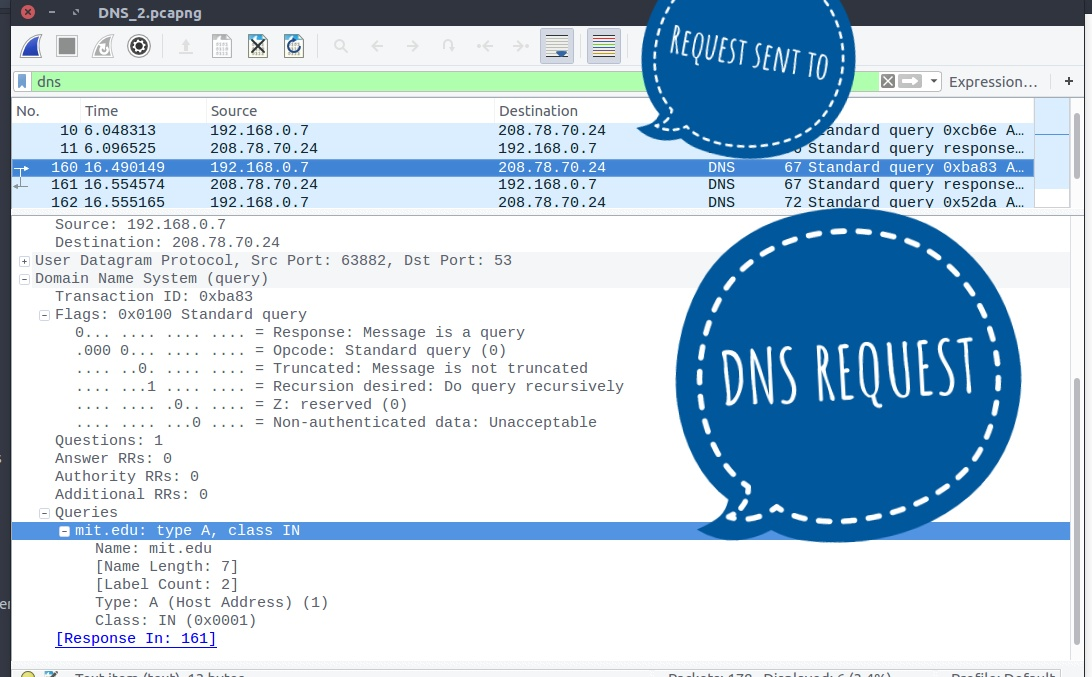
\includegraphics[scale=0.45]{2_3_1}\\[10pt] 
    \vspace{1cm}

    \noindent
    \textbf{\large Question 4}
    What is the response from the DNS server in packet \#160 ? 
    Did the server resolve the DNS request? Explain in brief.\\[10pt]
    \textbf{\large Answer}
    The response from DNS server is in packet \#160 where it refused to give answer of query. No DNS server did ot resolve the DNS request.\\
    Here are the flags in response which clears the answer of server more precisely:\\
    Flags: 0x8105 Standard query response, Refused\\
    1... .... .... .... = Response: Message is a response\\
    .000 0... .... .... = Opcode: Standard query (0)\\
    .... .0.. .... .... = Authoritative: Server is not an authority for domain\\
    .... ..0. .... .... = Truncated: Message is not truncated\\
    .... ...1 .... .... = Recursion desired: Do query recursively\\
    .... .... 0... .... = Recursion available: Server can't do recursive queries\\
    .... .... .0.. .... = Z: reserved (0)\\
    .... .... ..0. .... = Answer authenticated: Answer/authority portion was not authenticated by the server\\
    .... .... ...0 .... = Non-authenticated data: Unacceptable\\
    .... .... .... 0101 = Reply code: Refused (5)\\[10pt]
    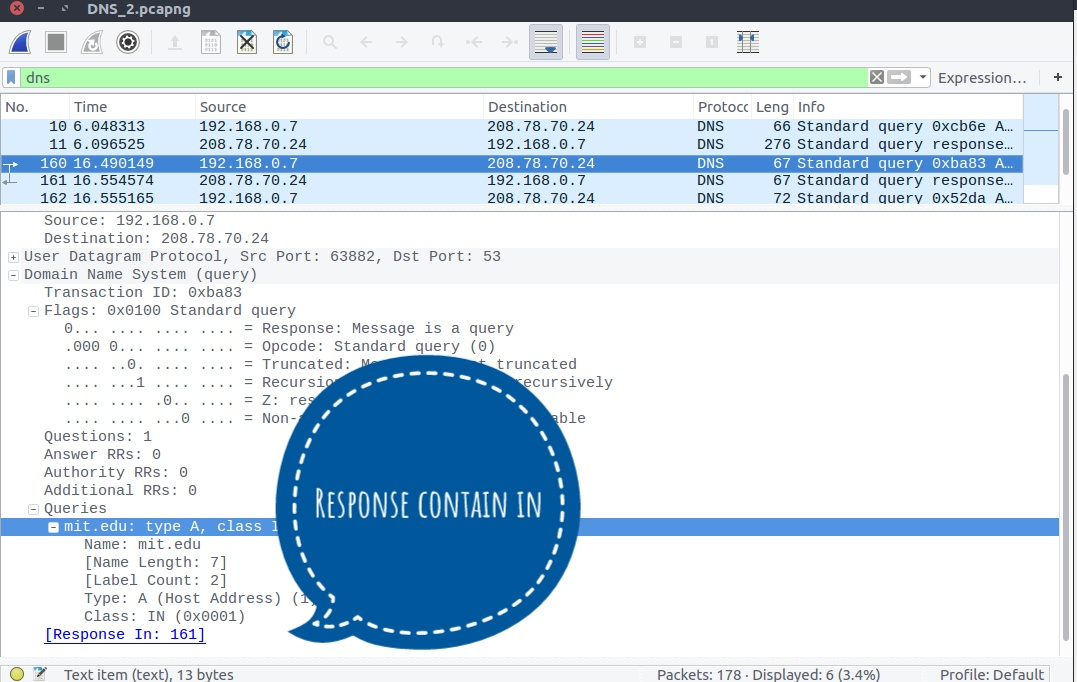
\includegraphics[scale=0.45]{2_4_1}\\[10pt] 
    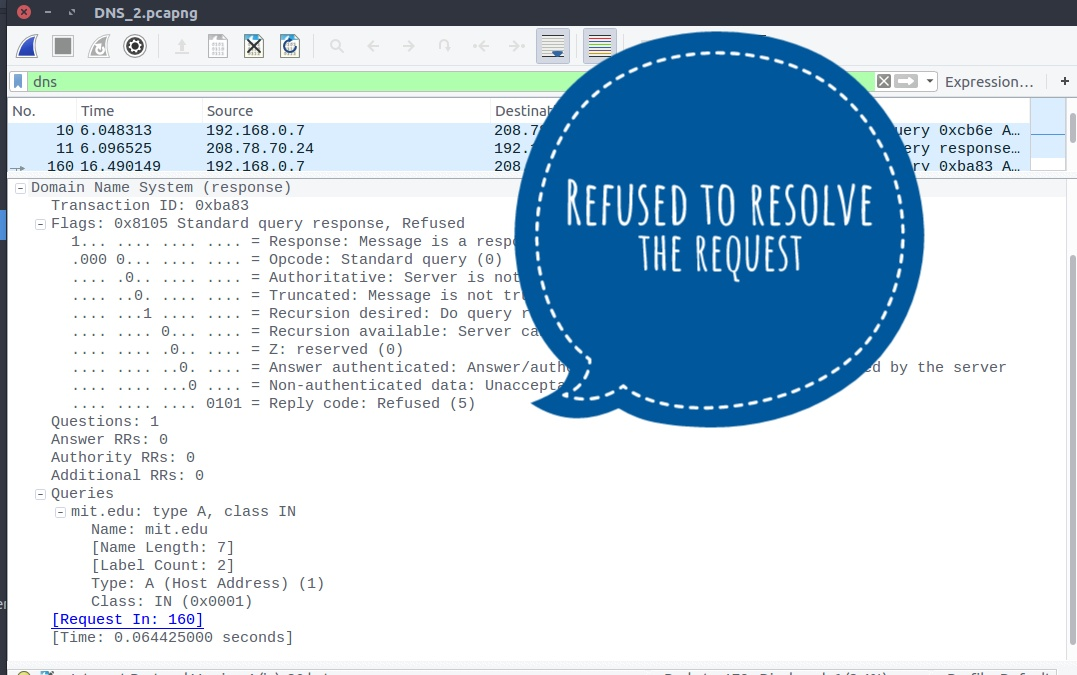
\includegraphics[scale=0.45]{2_4_2}\\[10pt] 
    \vspace{1cm}

    \begin{center}
        {\Large \textbf{SET 3: Working with the DNS 3.pcapng}}
    \end{center}

    \noindent
    \textbf{\large Question 1}
    To what IP address, is the DNS query sent in packet \#1? What "type" of DNS server is that?\\[10pt]
    \textbf{\large Answer}
    The destination IP address of the server is 192.168.0.1. The DNS server type is "Local server".\\[10pt]
    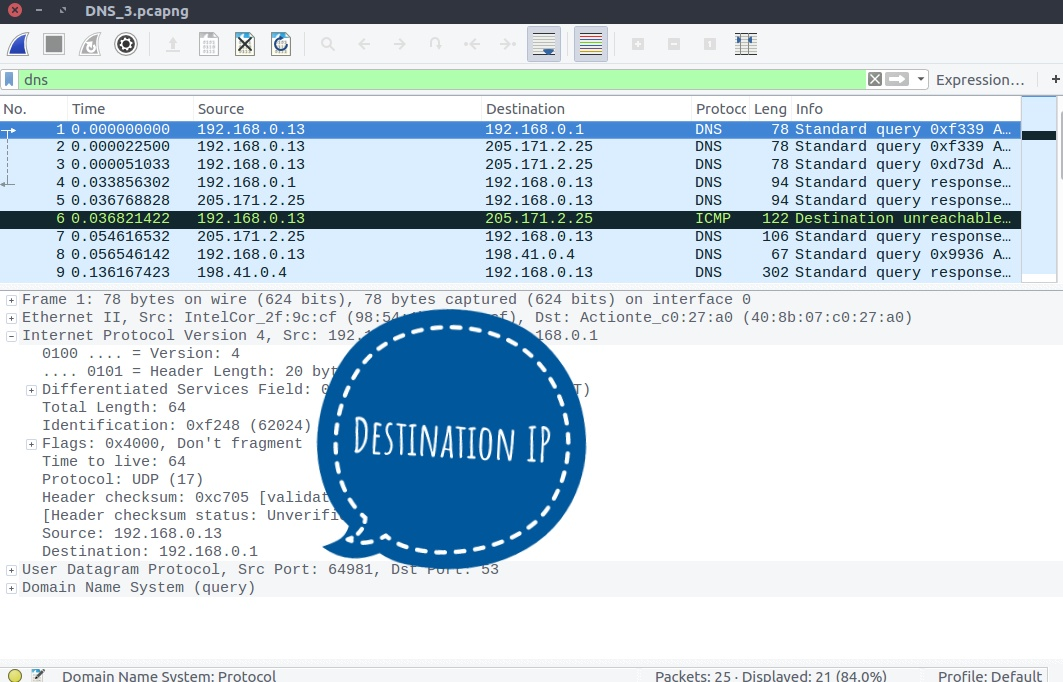
\includegraphics[scale=0.45]{3_1}\\[10pt]
    \vspace{1cm}

    \noindent
    \textbf{\large Question 2}
    To what IP address, is the DNS query sent in packet \#2? What "type" of DNS server is that?\\[10pt]
    \textbf{\large Answer}
    The destination IP address of the server is 205.171.2.25. The DNS server type is "Local server".\\[10pt]
    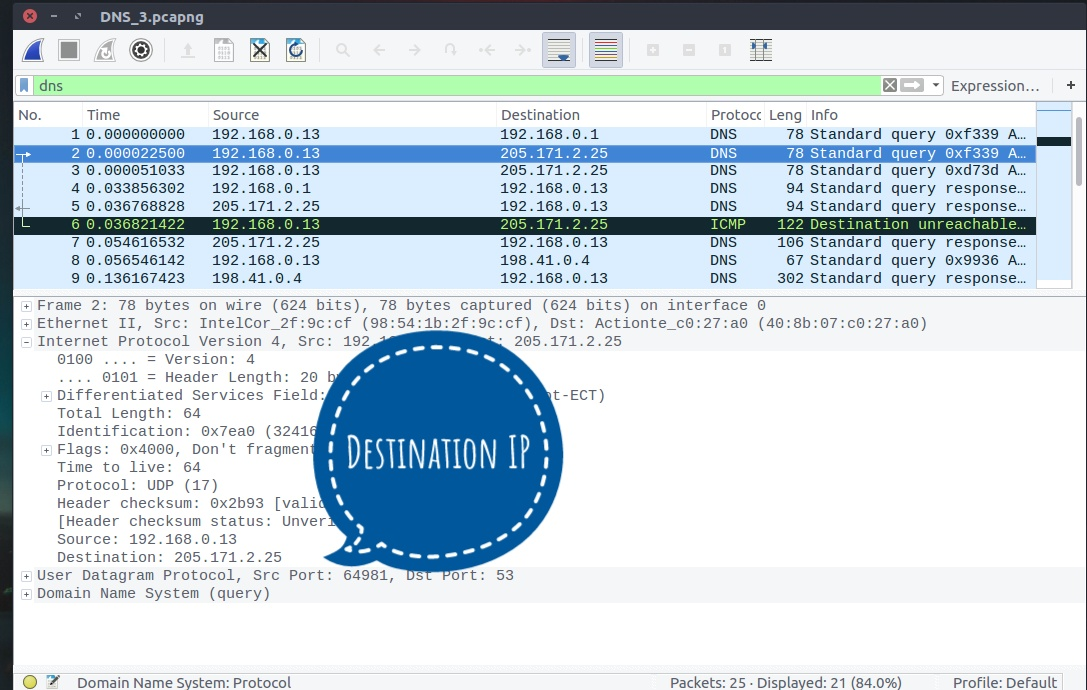
\includegraphics[scale=0.45]{3_2}\\[10pt]
    \vspace{1cm}

    \noindent
    \textbf{\large Question 3}
    Which packet contains the response of the query that is sent in packet \#2? What is your interpretation
of the response?\\[10pt]
    \textbf{\large Answer}
    The response of query in packet \#2 is contains in packet number \#5. The query has been resolved and answered.\\[10pt]
    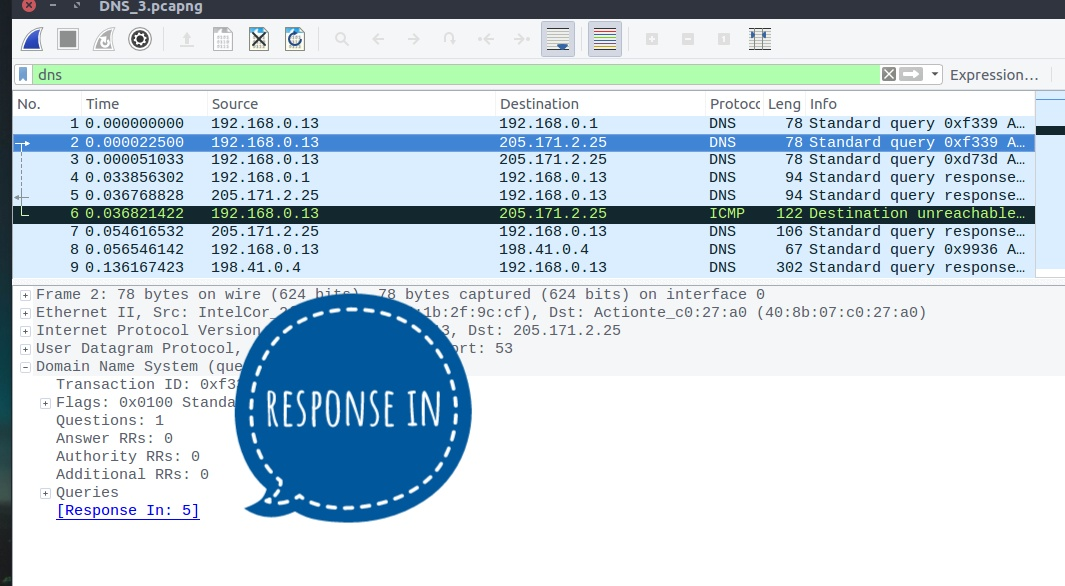
\includegraphics[scale=0.45]{3_3_1}\\[10pt]
    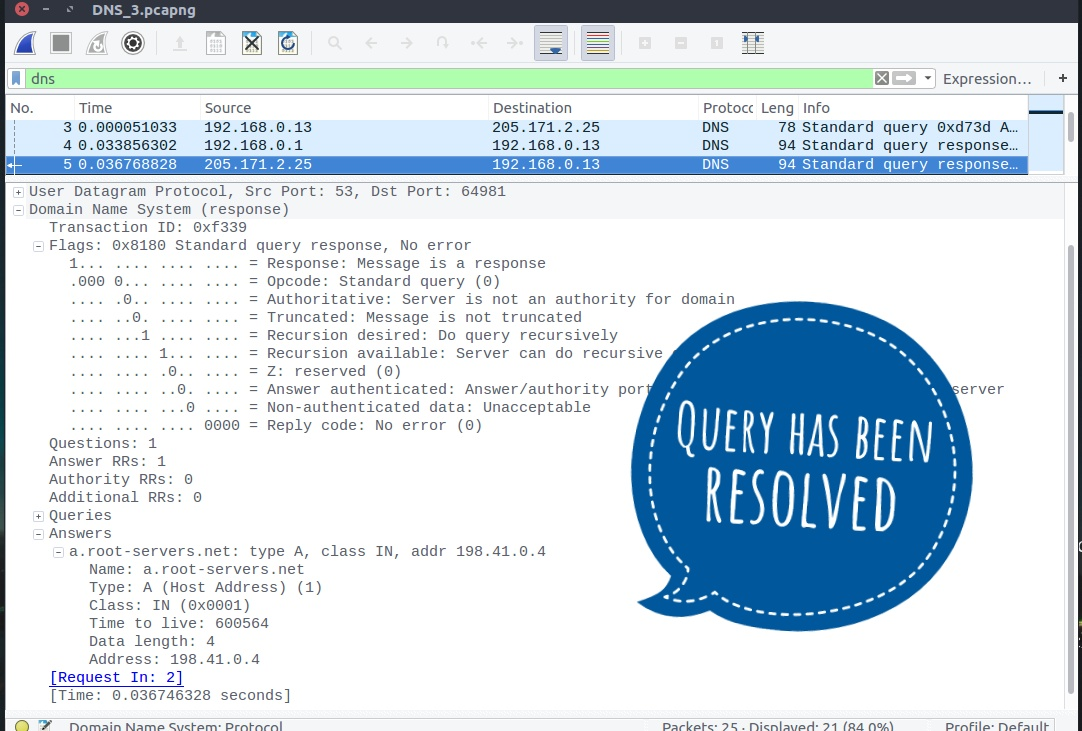
\includegraphics[scale=0.45]{3_3_2}\\[10pt]
    \vspace{1cm}

    \noindent
    \textbf{\large Question 4}
    What is the difference between query in packet \#2 and that in \#3 ?\\[10pt]
    \textbf{\large Answer}
    The difference between the queries is that packet \#2 have "type A" which gives IPv4 address, On the other hand, query in packet \#3 have "type AAAA" which gives IPv6 address in response.\\[10pt]
    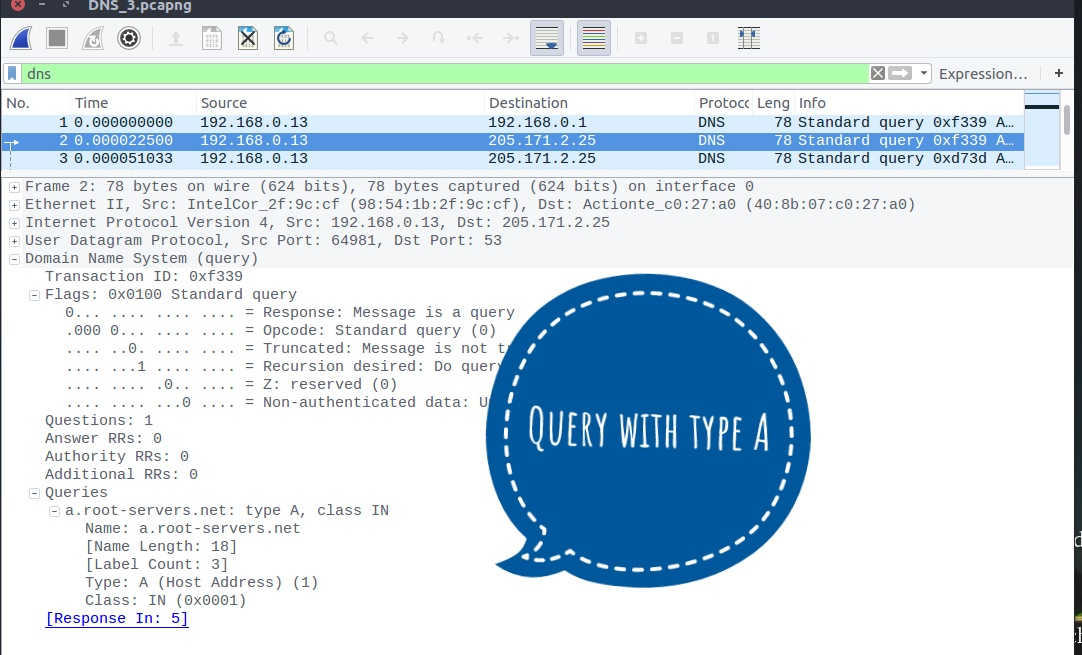
\includegraphics[scale=0.45]{3_4_1}\\[10pt]
    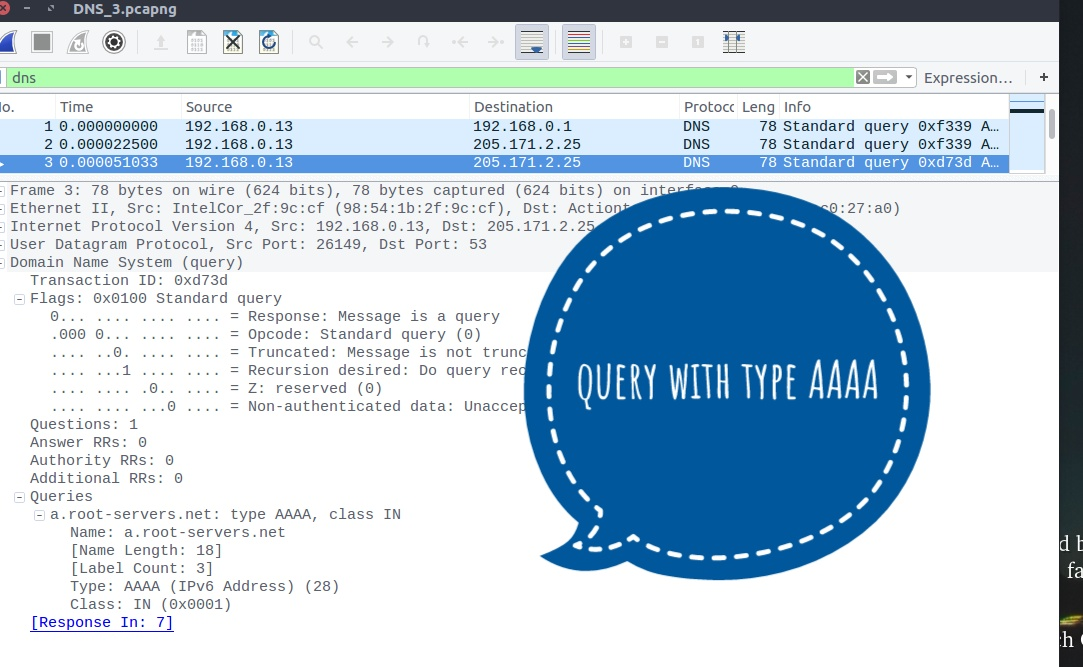
\includegraphics[scale=0.45]{3_4_2}\\[10pt]
    \vspace{1cm}

    \noindent
    \textbf{\large Question 5}
    What does the query in packet \#8 do? Which DNS server is being queried?\\[10pt]
    \textbf{\large Answer}
    Query in packet \#8 ask for IP address of "mit.edu". The server that has been queried is a.root-servers.net which is a root server.\\[10pt]
    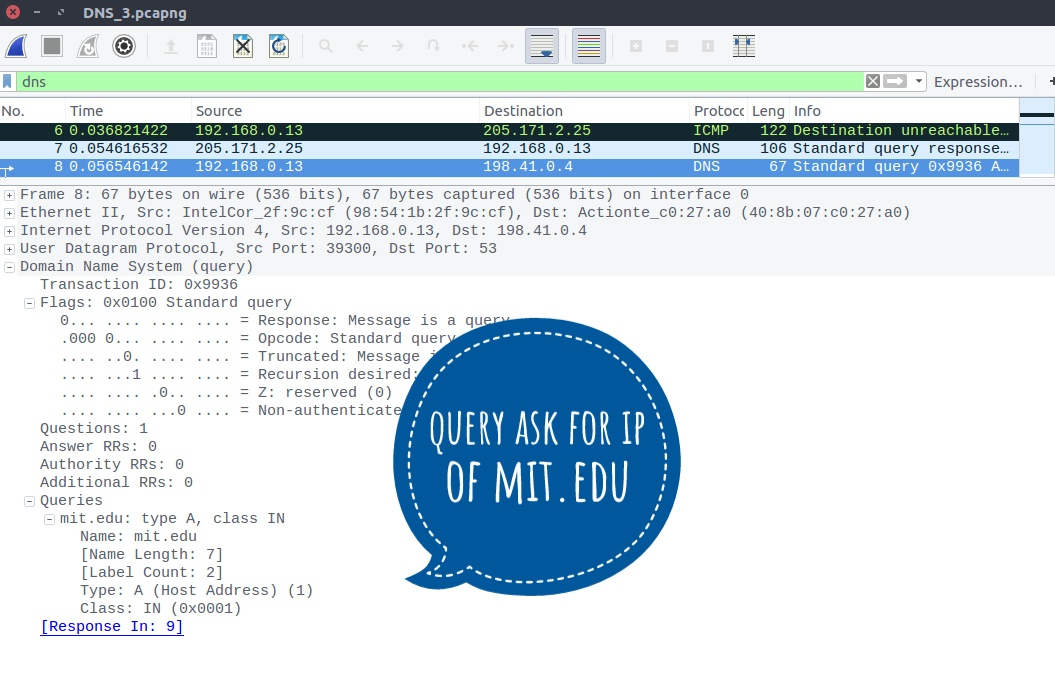
\includegraphics[scale=0.45]{3_5_1}\\[10pt]
    \vspace{1cm}

    \noindent
    \textbf{\large Question 6}
    Which packet contains the response of the query sent in packet \#8? What flags are set in this response?
Does it have the answer user wants? What information does it provide?\\[10pt]
    \textbf{\large Answer}
    The response of query sent in packet \#8 is in packet \#9.\\
    The flags in the response are:\\
    Flags: 0x8100 Standard query response, No error\\
    1... .... .... .... = Response: Message is a response\\
    .000 0... .... .... = Opcode: Standard query (0)\\
    .... .0.. .... .... = Authoritative: Server is not an authority for domain\\
    .... ..0. .... .... = Truncated: Message is not truncated\\
    .... ...1 .... .... = Recursion desired: Do query recursively\\
    .... .... 0... .... = Recursion available: Server can't do recursive queries\\
    .... .... .0.. .... = Z: reserved (0)\\
    .... .... ..0. .... = Answer authenticated: Answer/authority portion was not authenticated by the server\\
    .... .... ...0 .... = Non-authenticated data: Unacceptable\\
    .... .... .... 0000 = Reply code: No error (0)\\
    No it does not have answer which user wants. It provide information about which DNS servers have been tried to get answer of query.\\[10pt]
    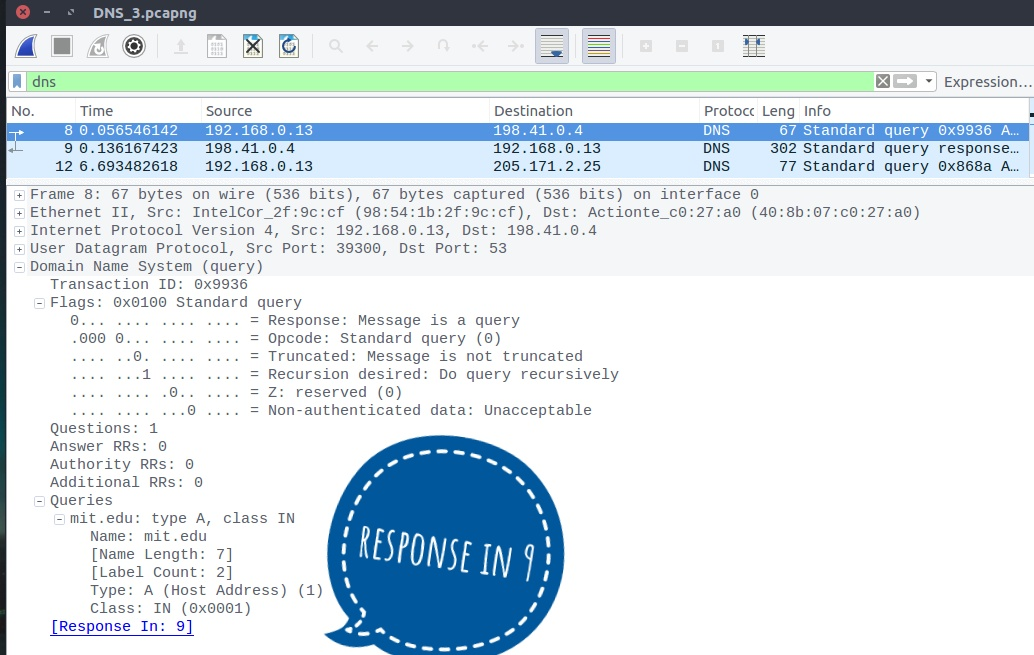
\includegraphics[scale=0.45]{3_6_1}\\[10pt]
    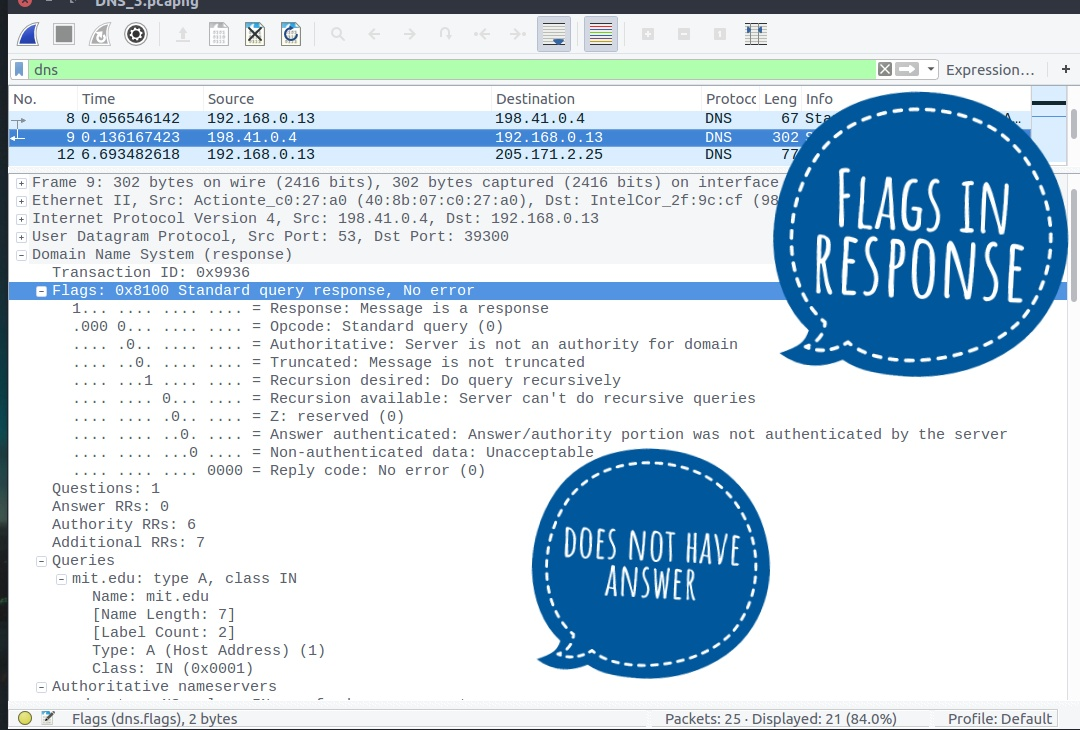
\includegraphics[scale=0.45]{3_6_2}\\[10pt]
    \vspace{1cm}


    \noindent
    \textbf{\large Question 7}
    Which DNS server is being queried in the query of packet \#16 ? Is it a local DNS server ?\\[10pt]
    \textbf{\large Answer}
    The server which has been quired is a.gtld-servers.net. No, it is not local server.\\[10pt]
    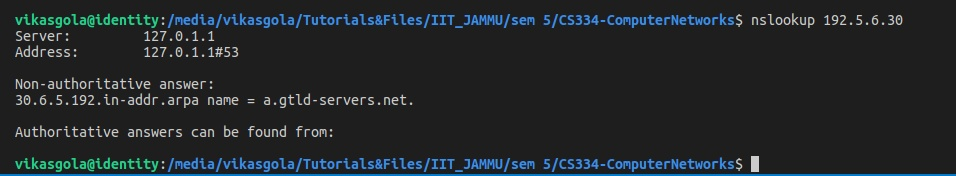
\includegraphics[scale=0.45]{3_7_1}\\[10pt]
    \vspace{1cm}

    \noindent
    \textbf{\large Question 8}
    Which packet contains the response of the query sent in packet \#16? What flags are set in this response?
Does it have the answer user wants? What information does it provide?\\[10pt]
    \textbf{\large Answer}
    The response of query of the packet \#16 is contains in packet \#17.\\
    The flags in the response is as follows:\\
    Flags: 0x8100 Standard query response, No error\\
    1... .... .... .... = Response: Message is a response\\
    .000 0... .... .... = Opcode: Standard query (0)\\
    .... .0.. .... .... = Authoritative: Server is not an authority for domain\\
    .... ..0. .... .... = Truncated: Message is not truncated\\
    .... ...1 .... .... = Recursion desired: Do query recursively\\
    .... .... 0... .... = Recursion available: Server can't do recursive queries\\
    .... .... .0.. .... = Z: reserved (0)\\
    .... .... ..0. .... = Answer authenticated: Answer/authority portion was not authenticated by the server\\
    .... .... ...0 .... = Non-authenticated data: Unacceptable\\
    .... .... .... 0000 = Reply code: No error (0)\\
    No, it does not have the answer which user wants. It provide information about which DNS servers have been tried to get answer of query.\\[10pt]
    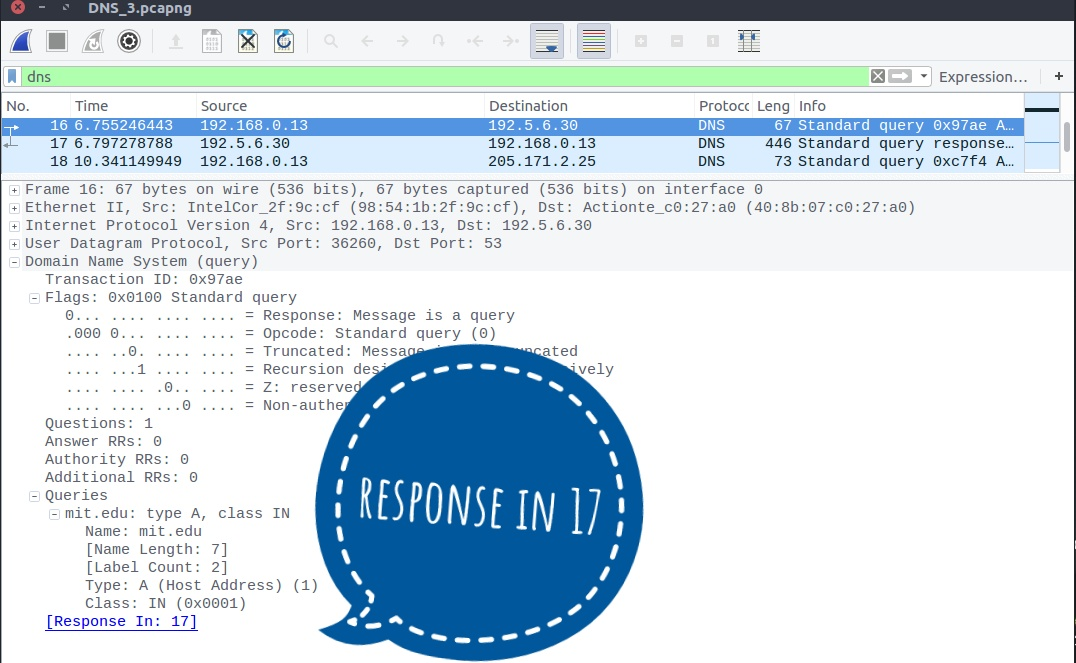
\includegraphics[scale=0.45]{3_8_1}\\[10pt]
    \vspace{1cm}


    \noindent
    \textbf{\large Question 9}
    What does the query in packet \#22 actually do? Which DNS server is being queried?\\[10pt]
    \textbf{\large Answer}
    Query in packet \#22 ask for IP address of "mit.edu". The server which has been quired is a14-64.akam.net.\\[10pt]
    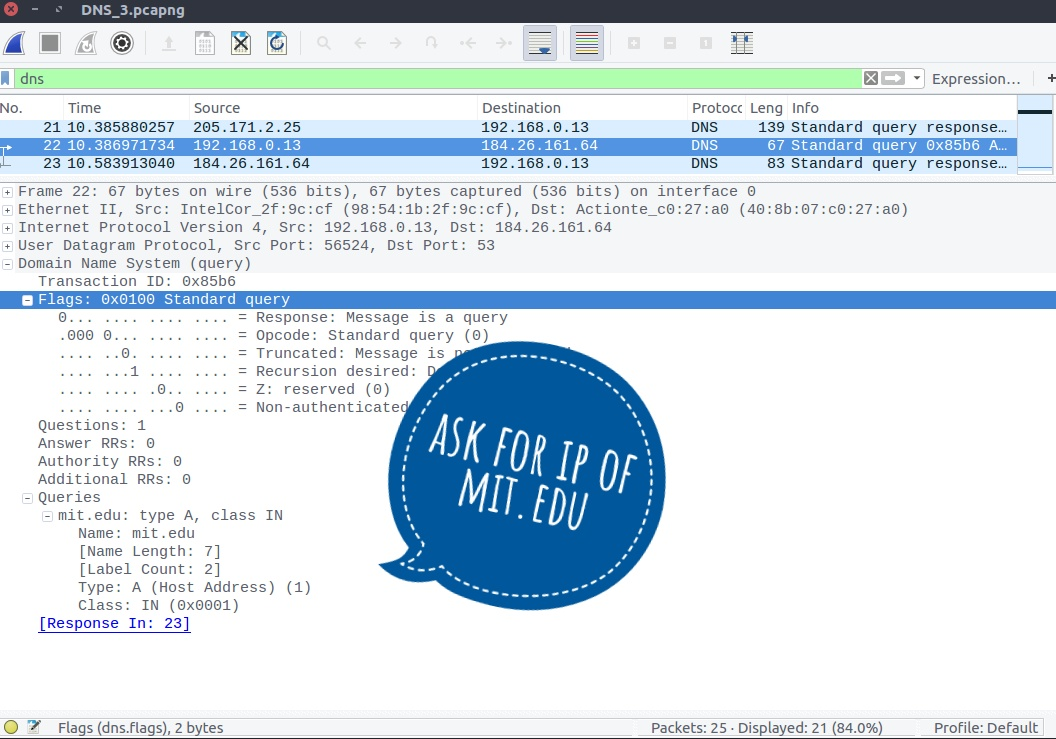
\includegraphics[scale=0.45]{3_9_1}\\[10pt]
    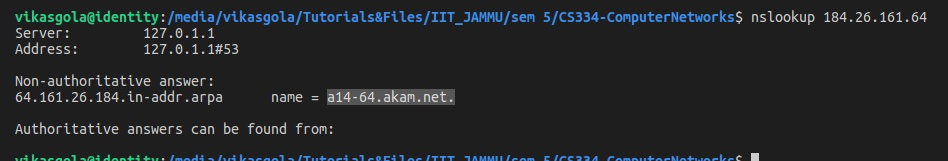
\includegraphics[scale=0.45]{3_9_2}\\[10pt]
    \vspace{1cm}


    \noindent
    \textbf{\large Question 10}
    Which packet contains the response to the query sent in packet \#22? What flags are set in this response?
Does it have the answer user wants? What information does it provide?\\[10pt]
    \textbf{\large Answer}
    The response of query of the packet \#22 is contains in packet \#23.\\
    The flags in the response is as follows:\\
    Flags: 0x8500 Standard query response, No error\\
    1... .... .... .... = Response: Message is a response\\
    .000 0... .... .... = Opcode: Standard query (0)\\
    .... .1.. .... .... = Authoritative: Server is an authority for domain\\
    .... ..0. .... .... = Truncated: Message is not truncated\\
    .... ...1 .... .... = Recursion desired: Do query recursively\\
    .... .... 0... .... = Recursion available: Server can't do recursive queries\\
    .... .... .0.. .... = Z: reserved (0)\\
    .... .... ..0. .... = Answer authenticated: Answer/authority portion was not authenticated by the server\\
    .... .... ...0 .... = Non-authenticated data: Unacceptable\\
    .... .... .... 0000 = Reply code: No error (0)\\
    Yes, it does have the answer which user wants. It provide information about IP address of "mit.edu".\\[10pt]
    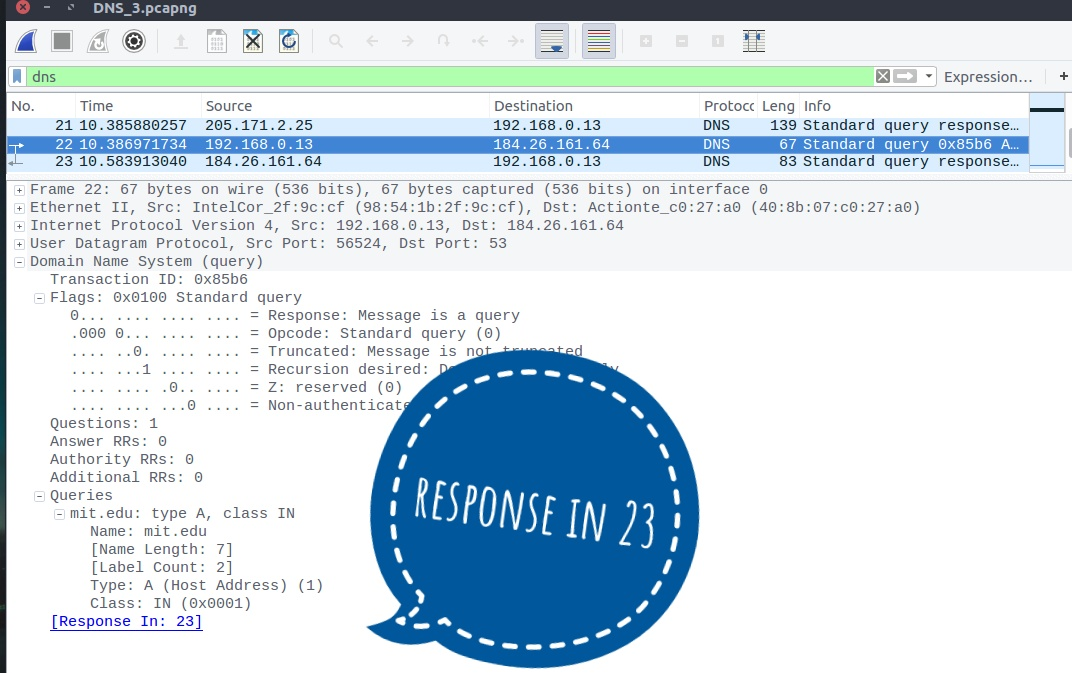
\includegraphics[scale=0.45]{3_10_1}\\[10pt]
    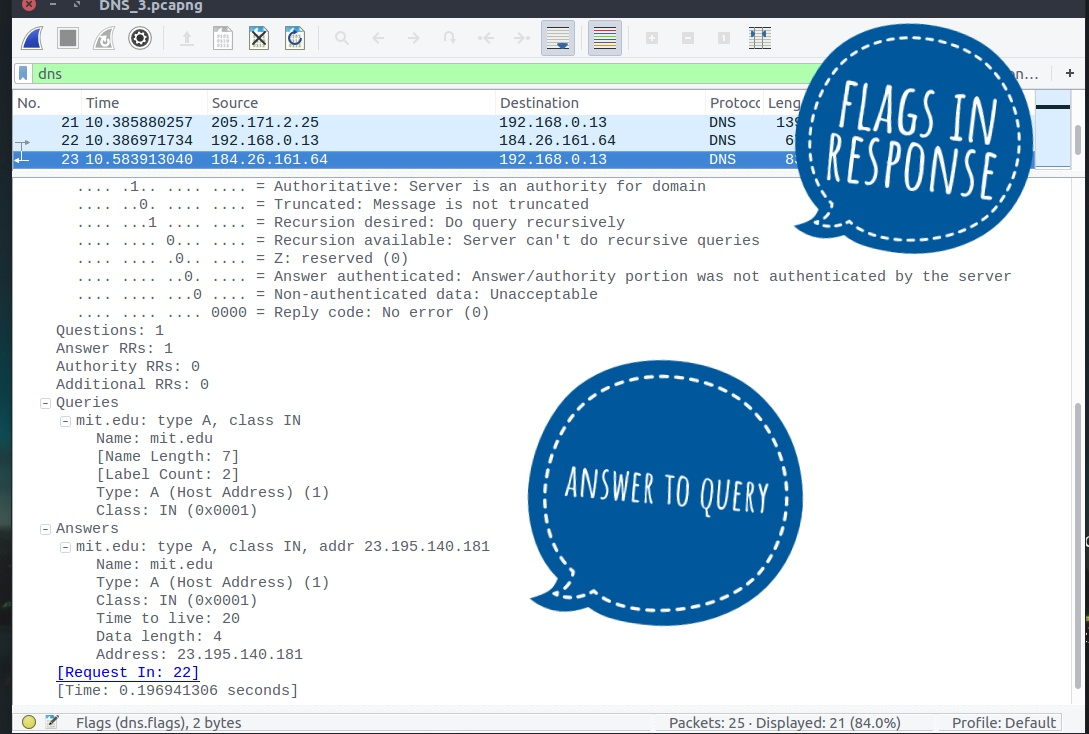
\includegraphics[scale=0.45]{3_10_2}\\[10pt]
    \vspace{1cm}
    
    \begin{center}
        {\Large \textbf{SET 4 - Using dig command}}
    \end{center}

    \noindent
    \textbf{\large Question 1}
    What is the dig command used to determine the authoritative DNS servers for www.mit.edu?\\[10pt]
    \textbf{\large Answer}
    The dig command used to determine the authoritative DNS servers for www.mit.edu is \textsf{dig mit.edu -t NS}.\\[10pt]
    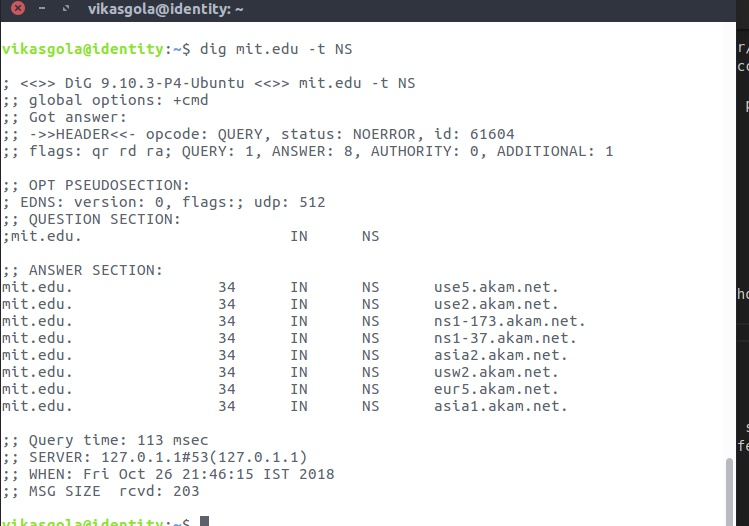
\includegraphics[scale=0.65]{4_1}
    \vspace{1cm}

    \noindent
    \textbf{\large Question 2}
    Using dig command determine the authoritative DNS servers for www.du.edu and www.ritchieschool.du.edu in a single dig command? Are DNS servers for both different?\\[10pt]
    \textbf{\large Answer}
    The dig command used to determine the authoritative DNS servers for www.du.edu and www.ritchieschool.du.edu is \textsf{ dig du.edu -t NS ritchieschool.du.edu -t NS}.
    Yes, both have different DNS servers.\\[10pt]
    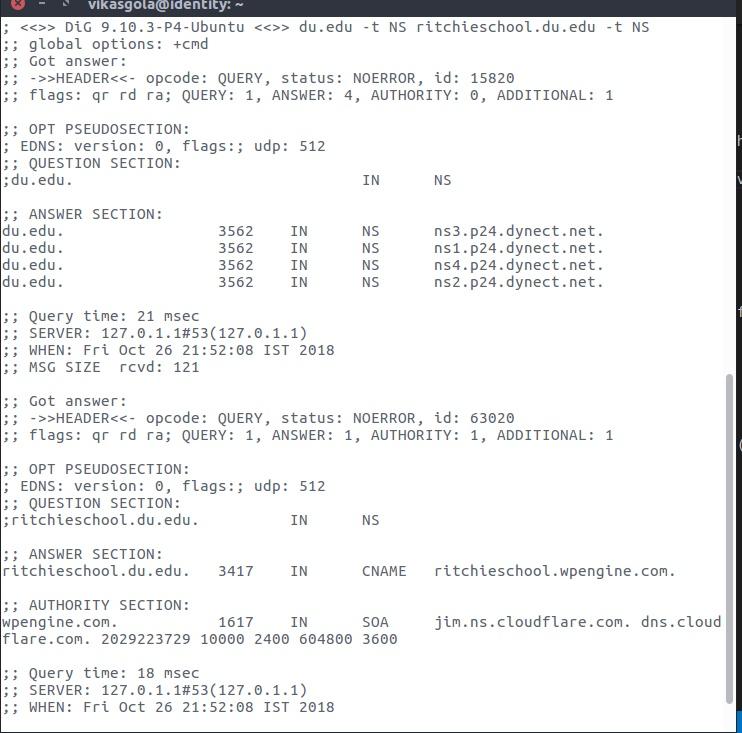
\includegraphics[scale=0.65]{4_2}
    \vspace{1cm}

    \noindent
    \textbf{\large Question 3}
    Use dig command with trace option to www.mit.edu (i.e. dig +trace www.mit.edu). What you can infer from the output?\\[10pt]
    \textbf{\large Answer}
    \\
    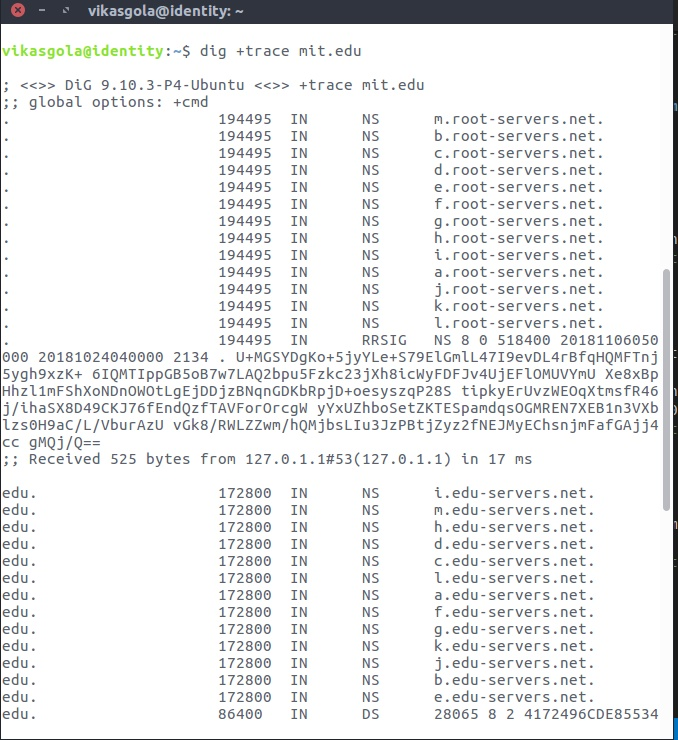
\includegraphics[scale=0.65]{4_3_1}\\[10pt]
    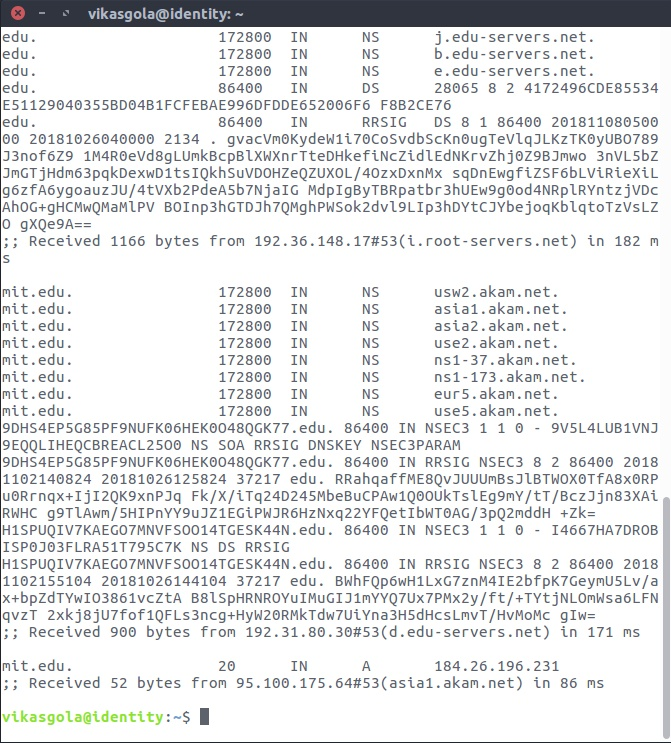
\includegraphics[scale=0.65]{4_3_2}\\[10pt]
    From the output we can see that this command is tracing how mit.edu domain is resolved from DNS servers.
    \vspace{1cm}


\end{document}